\documentclass[12pt]{article}
\usepackage[utf8]{inputenc}
\usepackage{amsmath,amsthm,amsfonts,amssymb}
\usepackage{tikz}
%\usepackage{subfig}
\usepackage[english]{babel}
%\usepackage{capt-of}
\newtheorem{theorem}{Theorem}
\usetikzlibrary{calc}
\usetikzlibrary{shapes}
\usepackage{hyperref}
%might be unnecessary
\usepackage{doi}
%bibliography CMDS


\usepackage{pdflscape}

\usepackage{filecontents}
\begin{filecontents*}{ohcrefs.bib}

@article{klarner_1967, 
title={Cell Growth Problems}, 
volume={19}, DOI={10.4153/CJM-1967-080-4}, 
journal={Canadian Journal of Mathematics}, 
publisher={Cambridge University Press}, 
author={Klarner, David A.}, 
year={1967}, 
pages={851–863}}

@misc{minecraftwiki, 
title={Tick}, 
url={https://minecraft.fandom.com/wiki/Tick}, 
journal={Minecraft Wiki}} 

@article{_api_ski_2019,
doi = {10.1016/j.jat.2019.105305},
url = {https://doi.org/10.1016%2Fj.jat.2019.105305},
year = 2019,
month = {dec},
publisher = {Elsevier {BV}
},
volume = {248},
pages = {105305},
author = {Tomasz M. {\L}api{\'{n}}ski},
title = {Multivariate Laplace's approximation with estimated error and application to limit theorems},
journal = {Journal of Approximation Theory}
}}

\end{filecontents*}

\usepackage[style=alphabetic]{biblatex}
\addbibresource{ohcrefs.bib}

%%% With amsthm package, creates environments for nicely formatted,
%%% labeled, and numbered propositions, etc.
\theoremstyle{plain}
\newtheorem{thm}{Theorem}
\newtheorem{lemma}[thm]{Lemma}
\newtheorem{prop}[thm]{Proposition}
\newtheorem{conj}[thm]{Conjecture}
\newtheorem{cor}[thm]{Corollary}
\newtheorem{claim}[thm]{Claim}
\newtheorem{fact}[thm]{Fact}

\theoremstyle{definition}
\newtheorem{eg}[thm]{Example}
\newtheorem{defn}[thm]{Definition}
\newtheorem{rem}[thm]{Remark}
\newtheorem{observ}[thm]{Observation}
\newtheorem{open}[thm]{Open Problem}
\newtheorem{prob.}[thm]{Problem}
\newtheorem{quest}[thm]{Question}

% I used these for making definitions and theorems, not what is above
\theoremstyle{remark}
\newtheorem{remark}[thm]{Remark}
\newtheorem{note}[thm]{Note}
\theoremstyle{definition}
\newtheorem{definition}{Definition}[section]
\newtheorem{exmp}{Example}[section]

\newcommand{\cellw}[4]{\draw[thick] ( #1 , #2 ) rectangle ( #3 , #4 );}
\newcommand{\cellb}[4]{\filldraw[black!60] ( #1 , #2 ) rectangle ( #3 , #4 ); \draw[thick] ( #1 , #2 ) rectangle ( #3 , #4 );}

\newcommand{\lablnode}[3]{\node[shape=circle,draw=white,fill=white, inner sep=0pt,minimum size=1pt] (A) at ( #1 , #2 ) {\{#3\}};}
\newcommand{\lablcell}[4]{\node[shape=circle,draw=white,fill=white, inner sep=0pt,minimum size=0.2cm] (A) at ( #1 , #2 ) {#3, #4};}

%nice quick solution
\usepackage[margin=1in]{geometry}

%doc info
\title{Minimal Inscribed Polyforms of the Extended Generalized Aztec Diamond}
\author{Jack Hanke}
\date{\today}

\begin{document}

\maketitle

Let the family of extended generalized aztec diamonds be denoted $A^{S^*}$. Below is an example of a polyform in $A^{S^*}_{5,3}$ and the labelled dual.

\begin{center}
    \begin{minipage}{0.45\textwidth}
        \centering
        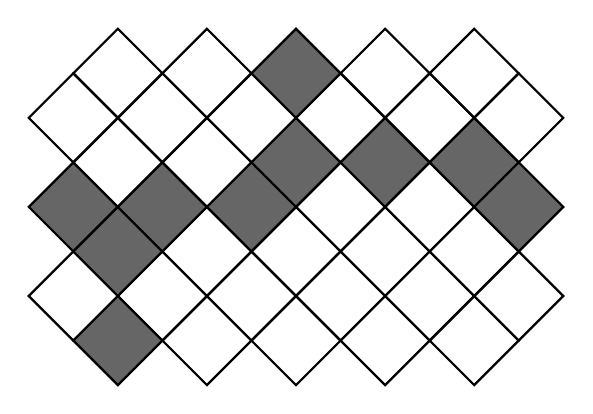
\begin{tikzpicture}[rotate=-45, scale=0.8]
            % row 1
            \cellw{2}{0}{3}{1}
            \cellb{3}{0}{4}{1}
            % row 2
            \cellb{1}{1}{2}{2}
            \cellb{2}{1}{3}{2}
            \cellw{3}{1}{4}{2}
            \cellw{4}{1}{5}{2}
            % row 3
            \cellw{0}{2}{1}{3}
            \cellw{1}{2}{2}{3}
            \cellb{2}{2}{3}{3}
            \cellw{3}{2}{4}{3}
            \cellw{4}{2}{5}{3}
            \cellw{5}{2}{6}{3}
            % row 4
            \cellw{0}{3}{1}{4}
            \cellw{1}{3}{2}{4}
            \cellw{2}{3}{3}{4}
            \cellb{3}{3}{4}{4}
            \cellw{4}{3}{5}{4}
            \cellw{5}{3}{6}{4}
            \cellw{6}{3}{7}{4}
            % row 5
            \cellw{1}{4}{2}{5}
            \cellw{2}{4}{3}{5}
            \cellb{3}{4}{4}{5}
            \cellw{4}{4}{5}{5}
            \cellw{5}{4}{6}{5}
            \cellw{6}{4}{7}{5}
            \cellw{7}{4}{8}{5}
            % row 6
            \cellb{2}{5}{3}{6}
            \cellw{3}{5}{4}{6}
            \cellb{4}{5}{5}{6}
            \cellw{5}{5}{6}{6}
            \cellw{6}{5}{7}{6}
            \cellw{7}{5}{8}{6}
    
            \cellw{3}{6}{4}{7}
            \cellw{4}{6}{5}{7}
            \cellb{5}{6}{6}{7}
            \cellb{6}{6}{7}{7}
    
            \cellw{4}{7}{5}{8}
            \cellw{5}{7}{6}{8}
        \end{tikzpicture}
    \end{minipage}
    \begin{minipage}{0.45\textwidth}
        \centering
        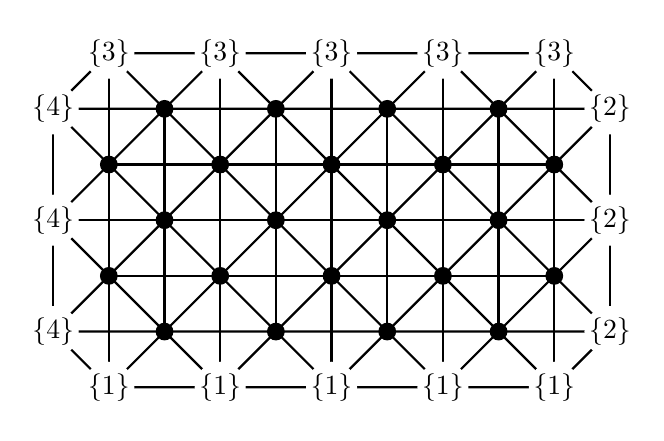
\begin{tikzpicture}[rotate=135]
        \draw[thick] (0,2) -- (0,3);
        \draw[thick] (1,1) -- (1,4);
        \draw[thick] (2,0) -- (2,5);
        \draw[thick] (3,0) -- (3,6);
        \draw[thick] (4,1) -- (4,7);
        \draw[thick] (5,2) -- (5,7);
        \draw[thick] (6,3) -- (6,6);
        \draw[thick] (7,4) -- (7,5);
        
        \draw[thick] (2,0) -- (3,0);
        \draw[thick] (1,1) -- (4,1);
        \draw[thick] (0,2) -- (5,2);
        \draw[thick] (0,3) -- (6,3);
        \draw[thick] (1,4) -- (7,4);
        \draw[thick] (2,5) -- (7,5);
        \draw[thick] (3,6) -- (6,6);
        \draw[thick] (4,7) -- (5,7);
        
        \draw[thick] (0,2) -- (2,0);
        \draw[thick] (0,3) -- (3,0);
        \draw[thick] (1,3) -- (3,1);
        \draw[thick] (1,4) -- (4,1);
        \draw[thick] (2,4) -- (4,2);
        \draw[thick] (2,5) -- (5,2);
        \draw[thick] (3,5) -- (5,3);
        \draw[thick] (3,6) -- (6,3);
        \draw[thick] (4,6) -- (6,4);
        \draw[thick] (4,7) -- (7,4);
        \draw[thick] (5,7) -- (7,5);
        
        
        \draw[thick] (0,3) -- (4,7);
        \draw[thick] (0,2) -- (5,7);
        \draw[thick] (1,2) -- (5,6);
        \draw[thick] (1,1) -- (6,6);
        \draw[thick] (2,1) -- (6,5);
        \draw[thick] (2,0) -- (7,5);
        \draw[thick] (3,0) -- (7,4);
        
        \( \lablnode{0}{2}{2} \)
        \( \lablnode{0}{3}{1} \)
        \( \lablnode{1}{1}{2} \)
        \draw[fill=black] (1,2) circle (3pt);
        \draw[fill=black] (1,3) circle (3pt);
        \( \lablnode{1}{4}{1} \)
        \( \lablnode{2}{0}{2} \)
        \draw[fill=black] (2,1) circle (3pt);
        \draw[fill=black] (2,2) circle (3pt);
        \draw[fill=black] (2,3) circle (3pt);
        \draw[fill=black] (2,4) circle (3pt);
        \( \lablnode{2}{5}{1} \)
        \( \lablnode{3}{0}{3} \)
        \draw[fill=black] (3,1) circle (3pt);
        \draw[fill=black] (3,2) circle (3pt);
        \draw[fill=black] (3,3) circle (3pt);
        \draw[fill=black] (3,4) circle (3pt);
        \draw[fill=black] (3,5) circle (3pt);
        \( \lablnode{3}{6}{1} \)
        \( \lablnode{4}{1}{3} \)
        \draw[fill=black] (4,2) circle (3pt);
        \draw[fill=black] (4,3) circle (3pt);
        \draw[fill=black] (4,4) circle (3pt);
        \draw[fill=black] (4,5) circle (3pt);
        \draw[fill=black] (4,6) circle (3pt);
        \( \lablnode{4}{7}{1} \)
        \( \lablnode{5}{2}{3} \)
        \draw[fill=black] (5,3) circle (3pt);
        \draw[fill=black] (5,4) circle (3pt);
        \draw[fill=black] (5,5) circle (3pt);
        \draw[fill=black] (5,6) circle (3pt);
        \( \lablnode{5}{7}{4} \)
        \( \lablnode{6}{3}{3} \)
        \draw[fill=black] (6,4) circle (3pt);
        \draw[fill=black] (6,5) circle (3pt);
        \( \lablnode{6}{6}{4} \)
        \( \lablnode{7}{4}{3} \)
        \( \lablnode{7}{5}{4} \)
    \end{tikzpicture}
    \end{minipage}
    % \captionof{figure}{The tiling and dual representation of $\triangle^{T}_3$ and an example polyform}
\end{center}

Note that $m(A^{S^*}_{n,m}) = n+m+2$. Some values of $\rho(A^{S^*}_{n,m})$ are summarized below.

\begin{table}[h]
    \centering
    \begin{tabular}{|c|c|c|c|c|c|}
        \hline
        $\rho(A^{S^*}_{n,m})$ & 1 & 2 & 3 & 4 & 5 \\
        \hline
        1 & 1 & 8 & 29 & 74 & 155 \\
        \hline
        2 & 8 & 68 & 266 & 752 & 1758 \\
         \hline
        3 & 29 & 266 & 1113 & 3428 & 8815\\
         \hline
        4 & 74 & 752 & 3428 & 11616 & 33036\\
         \hline
        5 & 155 & 1758 & 8815& 33036 & 104097\\
         \hline
    \end{tabular}
    \label{tab:uhh}
\end{table}

\begin{theorem}
    The generating function for the number of minimal inscribed polyforms in the extended generalized aztec diamond is

    \begin{eqnarray*}
        \sum_{n,m\geq 0} \rho(A^{S^*}_{n,m})x^n y^m & = & \\
        & & xy(2 \, x^{5} y - 11 \, x^{4} y^{2} + 9 \, x^{3} y^{3} - 11 \, x^{2} y^{4} + 2 \, x y^{5} \\
        & - & 10 \, x^{4} y + 16 \, x^{3} y^{2} + 16 \, x^{2} y^{3} - 10 \, x y^{4}\\
        & + & x^{4} + 15 \, x^{3} y - 21 \, x^{2} y^{2} + 15 \, x y^{3} + y^{4} - 8 \, x^{2} y - 8 \, x y^{2} \\
        & - & 4 \, x^{2} + 5 \, x y - 4 \, y^{2} + 2 \, x + 2 \, y + 1 ) \\
        & / & {\left(1 - 2 \, x - 2 \, y + x^{2} + x y + y^{2} \right)} {\left(1-x\right)}^{4} {\left(1-y\right)}^{4}
    \end{eqnarray*}

\end{theorem}

\begin{proof}

We first handle the $m=1$ case. $A^{S^*}_{4,1}$ is shown below as an example of what the $m=1$ case looks like.

\begin{center}
    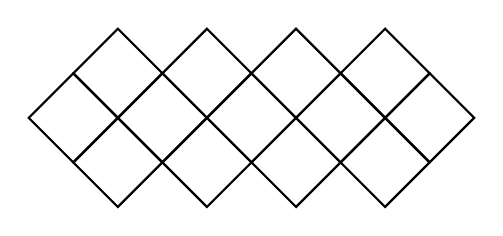
\begin{tikzpicture}[rotate=-45, scale=0.8]
        % row 1
        \cellw{2}{0}{3}{1}
        \cellw{3}{0}{4}{1}
        % row 2
        \cellw{2}{1}{3}{2}
        \cellw{3}{1}{4}{2}
        \cellw{4}{1}{5}{2}
        % row 3
        \cellw{3}{2}{4}{3}
        \cellw{4}{2}{5}{3}
        \cellw{5}{2}{6}{3}
        % row 4
        \cellw{4}{3}{5}{4}
        \cellw{5}{3}{6}{4}
        \cellw{6}{3}{7}{4}
        % row 5
        \cellw{5}{4}{6}{5}
        \cellw{6}{4}{7}{5}
    \end{tikzpicture}
\end{center}

We split the polyforms into the following distinct cases. First, the polyforms that include the following cells are enumerated by

\begin{center}
    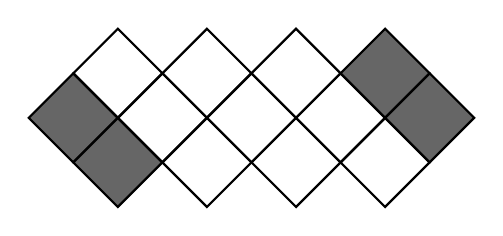
\begin{tikzpicture}[rotate=-45, scale=0.8]
        % row 1
        \cellb{2}{0}{3}{1}
        \cellb{3}{0}{4}{1}
        % row 2
        \cellw{2}{1}{3}{2}
        \cellw{3}{1}{4}{2}
        \cellw{4}{1}{5}{2}
        % row 3
        \cellw{3}{2}{4}{3}
        \cellw{4}{2}{5}{3}
        \cellw{5}{2}{6}{3}
        % row 4
        \cellw{4}{3}{5}{4}
        \cellw{5}{3}{6}{4}
        \cellw{6}{3}{7}{4}
        % row 5
        \cellb{5}{4}{6}{5}
        \cellb{6}{4}{7}{5}
    \end{tikzpicture}
\end{center}

$$\binom{n}{n-2}_2$$

Next we enumerate the polyforms of the following form

\begin{center}
    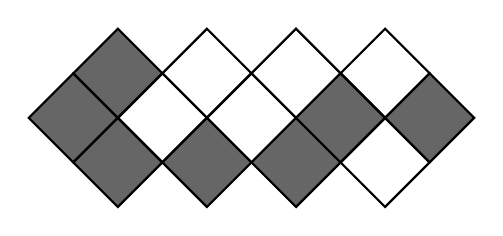
\begin{tikzpicture}[rotate=-45, scale=0.8]
        % row 1
        \cellb{2}{0}{3}{1}
        \cellb{3}{0}{4}{1}
        % row 2
        \cellb{2}{1}{3}{2}
        \cellw{3}{1}{4}{2}
        \cellb{4}{1}{5}{2}
        % row 3
        \cellw{3}{2}{4}{3}
        \cellw{4}{2}{5}{3}
        \cellb{5}{2}{6}{3}
        % row 4
        \cellw{4}{3}{5}{4}
        \cellb{5}{3}{6}{4}
        \cellw{6}{3}{7}{4}
        % row 5
        \cellw{5}{4}{6}{5}
        \cellb{6}{4}{7}{5}
    \end{tikzpicture}
\end{center}

$$(n-2)$$

Next we enumerate the polyforms of the following form

\begin{center}
    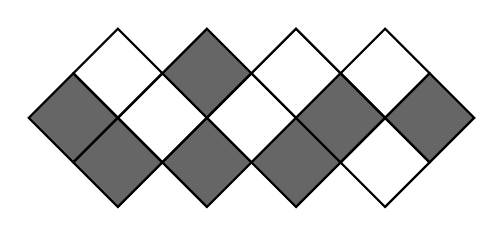
\begin{tikzpicture}[rotate=-45, scale=0.8]
        % row 1
        \cellb{2}{0}{3}{1}
        \cellb{3}{0}{4}{1}
        % row 2
        \cellw{2}{1}{3}{2}
        \cellw{3}{1}{4}{2}
        \cellb{4}{1}{5}{2}
        % row 3
        \cellb{3}{2}{4}{3}
        \cellw{4}{2}{5}{3}
        \cellb{5}{2}{6}{3}
        % row 4
        \cellw{4}{3}{5}{4}
        \cellb{5}{3}{6}{4}
        \cellw{6}{3}{7}{4}
        % row 5
        \cellw{5}{4}{6}{5}
        \cellb{6}{4}{7}{5}
    \end{tikzpicture}
\end{center}

$$\frac{(n-2)(n-3)}{2}$$

The single polyform below must be included.

\begin{center}
    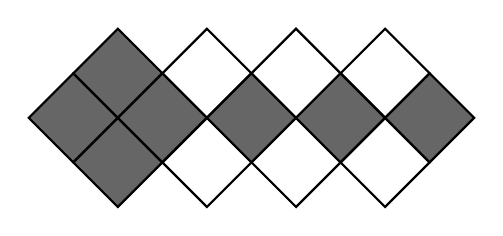
\begin{tikzpicture}[rotate=-45, scale=0.8]
        % row 1
        \cellb{2}{0}{3}{1}
        \cellb{3}{0}{4}{1}
        % row 2
        \cellb{2}{1}{3}{2}
        \cellb{3}{1}{4}{2}
        \cellw{4}{1}{5}{2}
        % row 3
        \cellw{3}{2}{4}{3}
        \cellb{4}{2}{5}{3}
        \cellw{5}{2}{6}{3}
        % row 4
        \cellw{4}{3}{5}{4}
        \cellb{5}{3}{6}{4}
        \cellw{6}{3}{7}{4}
        % row 5
        \cellw{5}{4}{6}{5}
        \cellb{6}{4}{7}{5}
    \end{tikzpicture}
\end{center}

$$1$$

Next we enumerate the polyforms of the following form

\begin{center}
    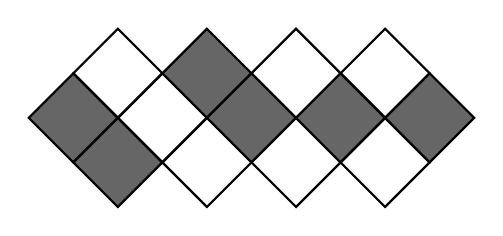
\begin{tikzpicture}[rotate=-45, scale=0.8]
        % row 1
        \cellb{2}{0}{3}{1}
        \cellb{3}{0}{4}{1}
        % row 2
        \cellw{2}{1}{3}{2}
        \cellw{3}{1}{4}{2}
        \cellw{4}{1}{5}{2}
        % row 3
        \cellb{3}{2}{4}{3}
        \cellb{4}{2}{5}{3}
        \cellw{5}{2}{6}{3}
        % row 4
        \cellw{4}{3}{5}{4}
        \cellb{5}{3}{6}{4}
        \cellw{6}{3}{7}{4}
        % row 5
        \cellw{5}{4}{6}{5}
        \cellb{6}{4}{7}{5}
    \end{tikzpicture}
\end{center}

$$ \sum_{k=2}^{n-1}\binom{k}{k-2}_2 $$

Finally, polyforms of this form are enumerated by 

\begin{center}
    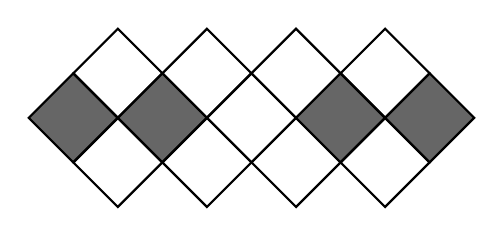
\begin{tikzpicture}[rotate=-45, scale=0.8]
        % row 1
        \cellb{2}{0}{3}{1}
        \cellw{3}{0}{4}{1}
        % row 2
        \cellw{2}{1}{3}{2}
        \cellb{3}{1}{4}{2}
        \cellw{4}{1}{5}{2}
        % row 3
        \cellw{3}{2}{4}{3}
        \cellw{4}{2}{5}{3}
        \cellw{5}{2}{6}{3}
        % row 4
        \cellw{4}{3}{5}{4}
        \cellb{5}{3}{6}{4}
        \cellw{6}{3}{7}{4}
        % row 5
        \cellw{5}{4}{6}{5}
        \cellb{6}{4}{7}{5}
    \end{tikzpicture}
\end{center}

$$\rho(A^{S^*}_{n-2,1})$$

Multiplying by the appropriate constants for reflections and rotations, and re-indexing, gives

\begin{equation*}
    \rho(A^{S^*}_{n+3,1}) = 2\binom{n+3}{n+1}_2 + 2(n+1)n + 2(n+1) + 2 + 4\sum_{k=2}^{n+2}\binom{k}{k-2}_2 + \rho(A^{S^*}_{n+1,1})
\end{equation*}

this can be solved using common techniques to get

\begin{equation*}
    \sum_{n \geq 1} \rho(A^{S^*}_{n,1}) x^n = \frac{x+3x^2-x^3-x^4}{(1-x)^5}.
\end{equation*}

For the $n,m \geq 2$ case, we begin by indexing the cells for reference. 
    
\begin{center}
    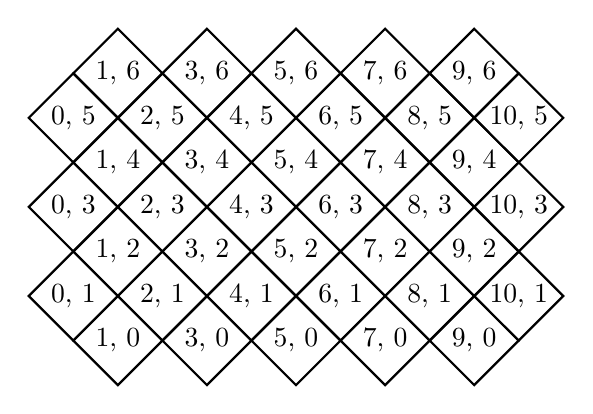
\begin{tikzpicture}[rotate=-45, scale=0.8]
        % row 1
        \lablcell{2.5}{0.5}{0}{1}
        \cellw{2}{0}{3}{1}
        \lablcell{3.5}{0.5}{1}{0}
        \cellw{3}{0}{4}{1}
        % row 2
        \lablcell{1.5}{1.5}{0}{3}
        \cellw{1}{1}{2}{2}
        \lablcell{2.5}{1.5}{1}{2}
        \cellw{2}{1}{3}{2}
        \lablcell{3.5}{1.5}{2}{1}
        \cellw{3}{1}{4}{2}
        \lablcell{4.5}{1.5}{3}{0}
        \cellw{4}{1}{5}{2}
        % row 3
        \lablcell{0.5}{2.5}{0}{5}
        \cellw{0}{2}{1}{3}
        \lablcell{1.5}{2.5}{1}{4}
        \cellw{1}{2}{2}{3}
        \lablcell{2.5}{2.5}{2}{3}
        \cellw{2}{2}{3}{3}
        \lablcell{3.5}{2.5}{3}{2}
        \cellw{3}{2}{4}{3}
        \lablcell{4.5}{2.5}{4}{1}
        \cellw{4}{2}{5}{3}
        \lablcell{5.5}{2.5}{5}{0}
        \cellw{5}{2}{6}{3}
        % row 4
        \lablcell{0.5}{3.5}{1}{6}
        \cellw{0}{3}{1}{4}
        \lablcell{1.5}{3.5}{2}{5}
        \cellw{1}{3}{2}{4}
        \lablcell{2.5}{3.5}{3}{4}
        \cellw{2}{3}{3}{4}
        \lablcell{3.5}{3.5}{4}{3}
        \cellw{3}{3}{4}{4}
        \lablcell{4.5}{3.5}{5}{2}
        \cellw{4}{3}{5}{4}
        \lablcell{5.5}{3.5}{6}{1}
        \cellw{5}{3}{6}{4}
        \lablcell{6.5}{3.5}{7}{0}
        \cellw{6}{3}{7}{4}
        % row 5
        \lablcell{1.5}{4.5}{3}{6}
        \cellw{1}{4}{2}{5}
        \lablcell{2.5}{4.5}{4}{5}
        \cellw{2}{4}{3}{5}
        \lablcell{3.5}{4.5}{5}{4}
        \cellw{3}{4}{4}{5}
        \lablcell{4.5}{4.5}{6}{3}
        \cellw{4}{4}{5}{5}
        \lablcell{5.5}{4.5}{7}{2}
        \cellw{5}{4}{6}{5}
        \lablcell{6.5}{4.5}{8}{1}
        \cellw{6}{4}{7}{5}
        \lablcell{7.5}{4.5}{9}{0}
        \cellw{7}{4}{8}{5}
        % row 6
        \lablcell{2.5}{5.5}{5}{6}
        \cellw{2}{5}{3}{6}
        \lablcell{3.5}{5.5}{6}{5}
        \cellw{3}{5}{4}{6}
        \lablcell{4.5}{5.5}{7}{4}
        \cellw{4}{5}{5}{6}
        \lablcell{5.5}{5.5}{8}{3}
        \cellw{5}{5}{6}{6}
        \lablcell{6.5}{5.5}{9}{2}
        \cellw{6}{5}{7}{6}
        \lablcell{7.5}{5.5}{10}{1}
        \lablcell{7.5}{5.5}{10}{1}
        \cellw{7}{5}{8}{6}
        
        \lablcell{3.5}{6.5}{7}{6}
        \cellw{3}{6}{4}{7}
        \lablcell{4.5}{6.5}{8}{5}
        \cellw{4}{6}{5}{7}
        \lablcell{5.5}{6.5}{9}{4}
        \cellw{5}{6}{6}{7}
        \lablcell{6.5}{6.5}{10}{3}
        \cellw{6}{6}{7}{7}
        
        \lablcell{4.5}{7.5}{9}{6}
        \cellw{4}{7}{5}{8}
        \lablcell{5.5}{7.5}{10}{5}
        \cellw{5}{7}{6}{8}
    \end{tikzpicture}
\end{center}

The path from a point $(i,j)$ and $(\hat{i},\hat{j})$ is
$$\binom{\frac{1}{2}((i-\hat{i})+(j-\hat{j}))}{\frac{1}{2}((i-\hat{i})-(j-\hat{j}))}_2$$

where $\binom{n}{k}$ is the $n,k$-th trinomial coefficient. From properties of tinomial coefficients we have 
$$F(x,y)=\sum_{n,m\geq 0}\binom{n+m}{n-m}_2 x^n y^m = \frac{1-x-y}{(1-x-y)^2 -xy}$$
$$G(x,y)=\sum_{n,m\geq 0}\binom{n+m+1}{n-m}_2 x^n y^m = \frac{1}{(1-x-y)^2 -xy}.$$

We first define $cc(n,m)$ to be the number of minimal inscribed polyforms that contain the following cells.

\begin{center}
    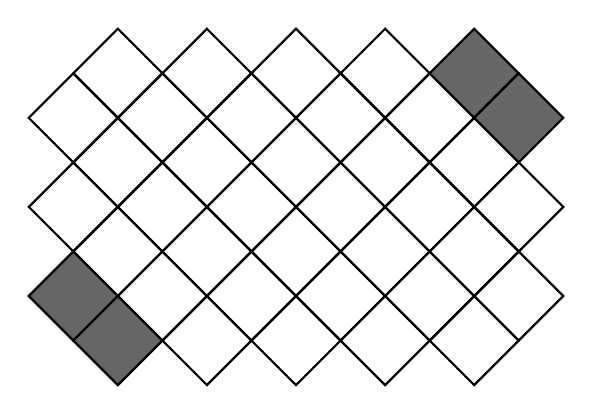
\begin{tikzpicture}[rotate=-45, scale=0.8]
        % row 1
        \cellb{2}{0}{3}{1}
        \cellb{3}{0}{4}{1}
        % row 2
        \cellw{1}{1}{2}{2}
        \cellw{2}{1}{3}{2}
        \cellw{3}{1}{4}{2}
        \cellw{4}{1}{5}{2}
        % row 3
        \cellw{0}{2}{1}{3}
        \cellw{1}{2}{2}{3}
        \cellw{2}{2}{3}{3}
        \cellw{3}{2}{4}{3}
        \cellw{4}{2}{5}{3}
        \cellw{5}{2}{6}{3}
        % row 4
        \cellw{0}{3}{1}{4}
        \cellw{1}{3}{2}{4}
        \cellw{2}{3}{3}{4}
        \cellw{3}{3}{4}{4}
        \cellw{4}{3}{5}{4}
        \cellw{5}{3}{6}{4}
        \cellw{6}{3}{7}{4}
        % row 5
        \cellw{1}{4}{2}{5}
        \cellw{2}{4}{3}{5}
        \cellw{3}{4}{4}{5}
        \cellw{4}{4}{5}{5}
        \cellw{5}{4}{6}{5}
        \cellw{6}{4}{7}{5}
        \cellw{7}{4}{8}{5}
        % row 6
        \cellw{2}{5}{3}{6}
        \cellw{3}{5}{4}{6}
        \cellw{4}{5}{5}{6}
        \cellw{5}{5}{6}{6}
        \cellw{6}{5}{7}{6}
        \cellw{7}{5}{8}{6}

        \cellw{3}{6}{4}{7}
        \cellw{4}{6}{5}{7}
        \cellw{5}{6}{6}{7}
        \cellw{6}{6}{7}{7}

        \cellb{4}{7}{5}{8}
        \cellb{5}{7}{6}{8}
    \end{tikzpicture}
\end{center}

It is easy to see that $$cc(n,m)=\binom{n+m-1}{n-m-1}_2 +\binom{n+m-1}{n-m+1}_2 -\binom{n+m-3}{n-m-1}_2 -\binom{n+m-3}{n-m+1}_2$$
for $n,m$ and $cc(n,1)=\binom{n}{n-2}_2$ and $cc(n,0)=1$. This gives

$$CC(x,y)=\sum_{n,m\geq 0}cc(n,m)x^n y^m = (1-xy)(1+(x+y)F(x,y))$$

We next define $c$ to be the number of polyforms that contain the following cells that are not counted in $cc$.

\begin{center}
    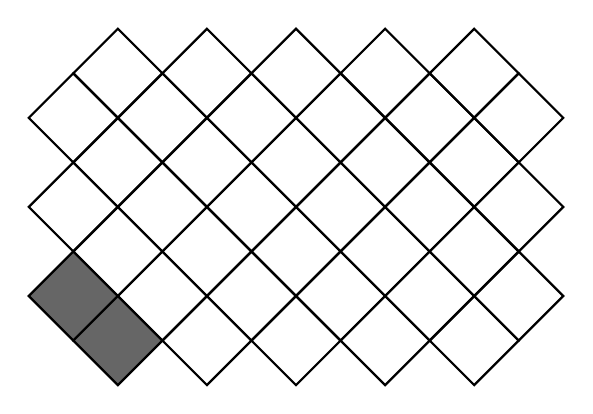
\begin{tikzpicture}[rotate=-45, scale=0.8]
        % row 1
        \cellb{2}{0}{3}{1}
        \cellb{3}{0}{4}{1}
        % row 2
        \cellw{1}{1}{2}{2}
        \cellw{2}{1}{3}{2}
        \cellw{3}{1}{4}{2}
        \cellw{4}{1}{5}{2}
        % row 3
        \cellw{0}{2}{1}{3}
        \cellw{1}{2}{2}{3}
        \cellw{2}{2}{3}{3}
        \cellw{3}{2}{4}{3}
        \cellw{4}{2}{5}{3}
        \cellw{5}{2}{6}{3}
        % row 4
        \cellw{0}{3}{1}{4}
        \cellw{1}{3}{2}{4}
        \cellw{2}{3}{3}{4}
        \cellw{3}{3}{4}{4}
        \cellw{4}{3}{5}{4}
        \cellw{5}{3}{6}{4}
        \cellw{6}{3}{7}{4}
        % row 5
        \cellw{1}{4}{2}{5}
        \cellw{2}{4}{3}{5}
        \cellw{3}{4}{4}{5}
        \cellw{4}{4}{5}{5}
        \cellw{5}{4}{6}{5}
        \cellw{6}{4}{7}{5}
        \cellw{7}{4}{8}{5}
        % row 6
        \cellw{2}{5}{3}{6}
        \cellw{3}{5}{4}{6}
        \cellw{4}{5}{5}{6}
        \cellw{5}{5}{6}{6}
        \cellw{6}{5}{7}{6}
        \cellw{7}{5}{8}{6}
        % row 7
        \cellw{3}{6}{4}{7}
        \cellw{4}{6}{5}{7}
        \cellw{5}{6}{6}{7}
        \cellw{6}{6}{7}{7}
        % row 8
        \cellw{4}{7}{5}{8}
        \cellw{5}{7}{6}{8}
    \end{tikzpicture}
\end{center}

To compute $c$ we study subclasses $c_0,c_1,c_2,c_3$ so that $c(n,m)=c_0(n,m)+c_1(n,m)+c_2(n,m)+c_3(n,m).$

The subclass $c_0$ counts the number of polyforms that contain two corners and include the bottom most corner cells. An example polyform in $c_0$ can be found below. 

\begin{center}
    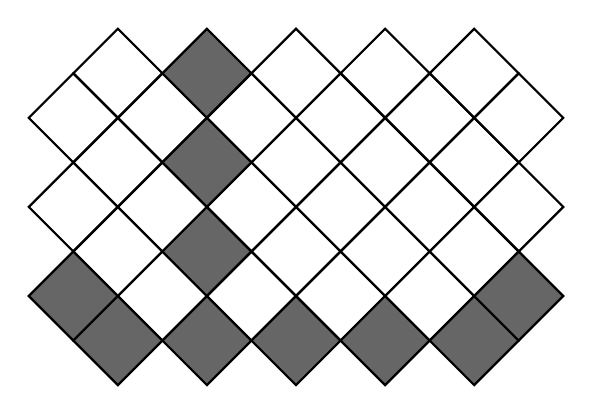
\begin{tikzpicture}[rotate=-45, scale=0.8]
        % row 1
        \cellb{2}{0}{3}{1}
        \cellb{3}{0}{4}{1}
        % row 2
        \cellw{1}{1}{2}{2}
        \cellw{2}{1}{3}{2}
        \cellw{3}{1}{4}{2}
        \cellb{4}{1}{5}{2}
        % row 3
        \cellw{0}{2}{1}{3}
        \cellw{1}{2}{2}{3}
        \cellw{2}{2}{3}{3}
        \cellb{3}{2}{4}{3}
        \cellw{4}{2}{5}{3}
        \cellb{5}{2}{6}{3}
        % row 4
        \cellw{0}{3}{1}{4}
        \cellw{1}{3}{2}{4}
        \cellb{2}{3}{3}{4}
        \cellw{3}{3}{4}{4}
        \cellw{4}{3}{5}{4}
        \cellw{5}{3}{6}{4}
        \cellb{6}{3}{7}{4}
        % row 5
        \cellb{1}{4}{2}{5}
        \cellw{2}{4}{3}{5}
        \cellw{3}{4}{4}{5}
        \cellw{4}{4}{5}{5}
        \cellw{5}{4}{6}{5}
        \cellw{6}{4}{7}{5}
        \cellb{7}{4}{8}{5}
        % row 6
        \cellw{2}{5}{3}{6}
        \cellw{3}{5}{4}{6}
        \cellw{4}{5}{5}{6}
        \cellw{5}{5}{6}{6}
        \cellw{6}{5}{7}{6}
        \cellb{7}{5}{8}{6}
        % row 7
        \cellw{3}{6}{4}{7}
        \cellw{4}{6}{5}{7}
        \cellw{5}{6}{6}{7}
        \cellw{6}{6}{7}{7}
        % row 8
        \cellw{4}{7}{5}{8}
        \cellw{5}{7}{6}{8}
    \end{tikzpicture}
\end{center}

We have that the generating function for $c_0$ is
$$C_0(x,y)=\frac{}x^3y^2{(1-x)^2 (1-y)} + \frac{}x^2y^3{(1-x) (1-y)^2}.$$

The subclass $c_1$ counts the number of polyforms that contain the ``thin u" substructure. The substructure and an example polyform in $c_1$ can be found below. 

\begin{center}
    \begin{minipage}{0.45\textwidth}
        \centering
        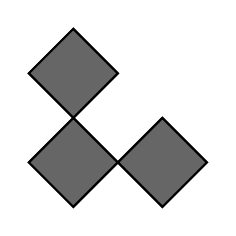
\begin{tikzpicture}[rotate=-45, scale=0.8]
            % row 1
            \cellb{2}{0}{3}{1}
            % row 2
            \cellb{1}{1}{2}{2}
            \cellb{3}{1}{4}{2}
        \end{tikzpicture}
    \end{minipage}
    \begin{minipage}{0.45\textwidth}
        \centering
        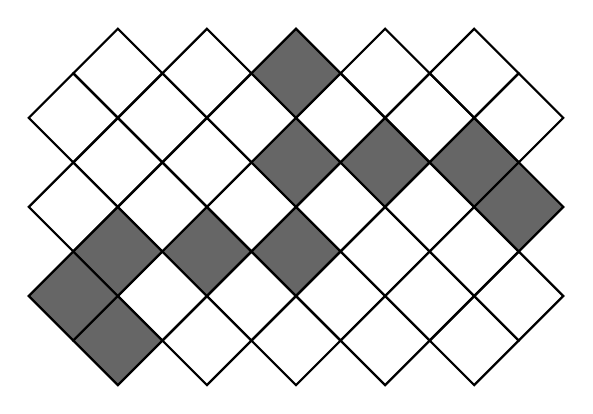
\begin{tikzpicture}[rotate=-45, scale=0.8]
            % row 1
            \cellb{2}{0}{3}{1}
            \cellb{3}{0}{4}{1}
            % row 2
            \cellw{1}{1}{2}{2}
            \cellb{2}{1}{3}{2}
            \cellw{3}{1}{4}{2}
            \cellw{4}{1}{5}{2}
            % row 3
            \cellw{0}{2}{1}{3}
            \cellw{1}{2}{2}{3}
            \cellw{2}{2}{3}{3}
            \cellb{3}{2}{4}{3}
            \cellw{4}{2}{5}{3}
            \cellw{5}{2}{6}{3}
            % row 4
            \cellw{0}{3}{1}{4}
            \cellw{1}{3}{2}{4}
            \cellw{2}{3}{3}{4}
            \cellw{3}{3}{4}{4}
            \cellb{4}{3}{5}{4}
            \cellw{5}{3}{6}{4}
            \cellw{6}{3}{7}{4}
            % row 5
            \cellw{1}{4}{2}{5}
            \cellw{2}{4}{3}{5}
            \cellb{3}{4}{4}{5}
            \cellw{4}{4}{5}{5}
            \cellw{5}{4}{6}{5}
            \cellw{6}{4}{7}{5}
            \cellw{7}{4}{8}{5}
            % row 6
            \cellb{2}{5}{3}{6}
            \cellw{3}{5}{4}{6}
            \cellb{4}{5}{5}{6}
            \cellw{5}{5}{6}{6}
            \cellw{6}{5}{7}{6}
            \cellw{7}{5}{8}{6}
            % row 7
            \cellw{3}{6}{4}{7}
            \cellw{4}{6}{5}{7}
            \cellb{5}{6}{6}{7}
            \cellb{6}{6}{7}{7}
            % row 8
            \cellw{4}{7}{5}{8}
            \cellw{5}{7}{6}{8}
        \end{tikzpicture}
    \end{minipage}
    % \captionof{figure}{The tiling and dual representation of $\triangle^{T}_3$ and an example polyform}
\end{center}

This subclass can be counted with the following sums.
\begin{eqnarray*}
c_1(n,m) & = & 2\sum_{\substack{0\leq i\leq n-1 \\ 1\leq j\leq m-1}} \binom{i+j}{i-j}_2(n-1-i) + 2\sum_{\substack{0\leq i\leq n-1 \\ 0\leq j\leq m-3}} \binom{i+j+1}{i-j}_2(n-1-i) \\
& + & {} 2\sum_{\substack{1\leq i\leq n-1 \\ 0\leq j\leq m-1}} \binom{i+j}{i-j}_2(m-1-j) + 2\sum_{\substack{0\leq i\leq n-3 \\ 0\leq j\leq m-1}} \binom{i+j+1}{i-j}_2(m-1-j)),
\end{eqnarray*}
and has the following generating function
\begin{eqnarray*}
    C_1(x,y) & = &  \frac{2xy}{(1-x)(1-y)}\left(F(x,y)\left(\frac{x}{1-x}+\frac{y}{1-y}\right)+G(x,y)\left(\frac{xy^2}{1-x}+\frac{x^2y}{1-y}\right)  \right) \\
    & - & \frac{2x^2y}{(1-x)^3(1-y)} - \frac{2xy^2}{(1-x)(1-y)^3}.
\end{eqnarray*}
% $$C_1(x,y)=\frac{2xy}{(1-x)(1-y)}\left(F(x,y)\left(\frac{x}{1-x}+\frac{y}{1-y}\right)+G(x,y)\left(\frac{xy^2}{1-x}+\frac{x^2y}{1-y}\right)  \right) - \frac{2x^2y}{(1-x)^3(1-y)} - \frac{2xy^2}{(1-x)(1-y)^3}.$$

The subclass $c_2$ counts the number of polyforms that contain the ``thick u" substructure. The substructure and an example polyform in $c_1$ can be found below. 

\begin{center}
    \begin{minipage}{0.45\textwidth}
        \centering
        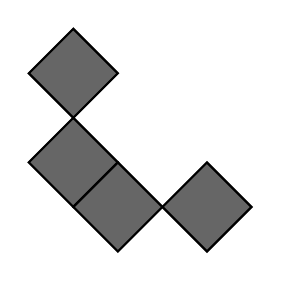
\begin{tikzpicture}[rotate=-45, scale=0.8]
            % row 1
            \cellb{2}{0}{3}{1}
            \cellb{3}{0}{4}{1}
            % row 2
            \cellb{1}{1}{2}{2}
            \cellb{4}{1}{5}{2}
        \end{tikzpicture}
    \end{minipage}
    \begin{minipage}{0.45\textwidth}
        \centering
        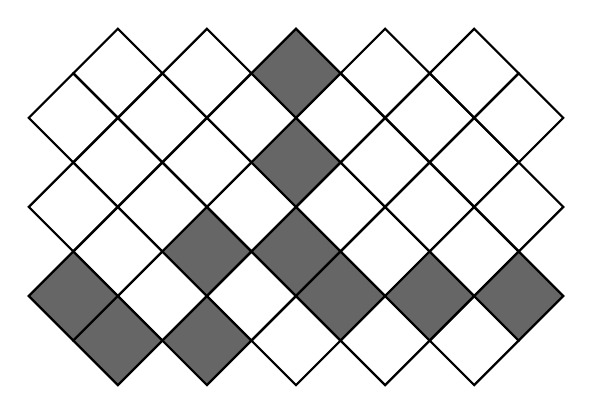
\begin{tikzpicture}[rotate=-45, scale=0.8]
            % row 1
            \cellb{2}{0}{3}{1}
            \cellb{3}{0}{4}{1}
            % row 2
            \cellw{1}{1}{2}{2}
            \cellw{2}{1}{3}{2}
            \cellw{3}{1}{4}{2}
            \cellb{4}{1}{5}{2}
            % row 3
            \cellw{0}{2}{1}{3}
            \cellw{1}{2}{2}{3}
            \cellw{2}{2}{3}{3}
            \cellb{3}{2}{4}{3}
            \cellw{4}{2}{5}{3}
            \cellw{5}{2}{6}{3}
            % row 4
            \cellw{0}{3}{1}{4}
            \cellw{1}{3}{2}{4}
            \cellw{2}{3}{3}{4}
            \cellw{3}{3}{4}{4}
            \cellb{4}{3}{5}{4}
            \cellb{5}{3}{6}{4}
            \cellw{6}{3}{7}{4}
            % row 5
            \cellw{1}{4}{2}{5}
            \cellw{2}{4}{3}{5}
            \cellb{3}{4}{4}{5}
            \cellw{4}{4}{5}{5}
            \cellw{5}{4}{6}{5}
            \cellb{6}{4}{7}{5}
            \cellw{7}{4}{8}{5}
            % row 6
            \cellb{2}{5}{3}{6}
            \cellw{3}{5}{4}{6}
            \cellw{4}{5}{5}{6}
            \cellw{5}{5}{6}{6}
            \cellw{6}{5}{7}{6}
            \cellb{7}{5}{8}{6}
            % row 7
            \cellw{3}{6}{4}{7}
            \cellw{4}{6}{5}{7}
            \cellw{5}{6}{6}{7}
            \cellw{6}{6}{7}{7}
            % row 8
            \cellw{4}{7}{5}{8}
            \cellw{5}{7}{6}{8}
        \end{tikzpicture}
    \end{minipage}
    % \captionof{figure}{The tiling and dual representation of $\triangle^{T}_3$ and an example polyform}
\end{center}

The subclass can be counted by the following sum
$c_2(n,m)=\sum_{\substack{1\leq i\leq n \\ 1\leq j\leq m \\ i,j \neq (1,1) \\ i,j \neq (n,m)}}cc(i,j),$
and has the following generating function
$$C_2(x,y) = \left(\frac{1}{(1-x)(1-y)}-1\right)\left(CC(x,y)-\frac{x}{1-x}-\frac{y}{1-y}-2\right)+\frac{x}{1-x}+\frac{y}{1-y}+xy.$$

Finally, the $c_3$ subclass counts the number of polyforms that contain ``u" and ``t" polyforms that don't include an adjacent corner. An example polyform can be found below.

\begin{center}
    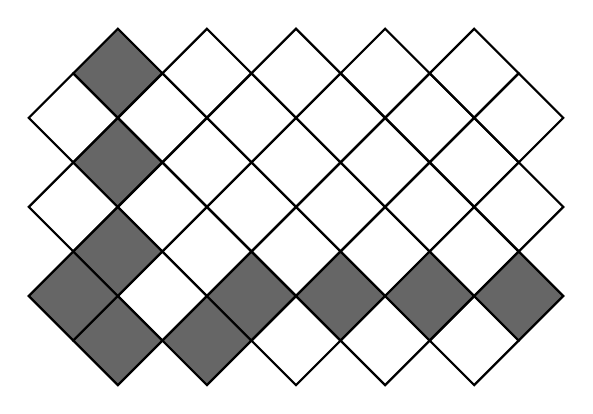
\begin{tikzpicture}[rotate=-45, scale=0.8]
        % row 1
        \cellb{2}{0}{3}{1}
        \cellb{3}{0}{4}{1}
        % row 2
        \cellw{1}{1}{2}{2}
        \cellb{2}{1}{3}{2}
        \cellw{3}{1}{4}{2}
        \cellb{4}{1}{5}{2}
        % row 3
        \cellw{0}{2}{1}{3}
        \cellb{1}{2}{2}{3}
        \cellw{2}{2}{3}{3}
        \cellw{3}{2}{4}{3}
        \cellb{4}{2}{5}{3}
        \cellw{5}{2}{6}{3}
        % row 4
        \cellb{0}{3}{1}{4}
        \cellw{1}{3}{2}{4}
        \cellw{2}{3}{3}{4}
        \cellw{3}{3}{4}{4}
        \cellw{4}{3}{5}{4}
        \cellb{5}{3}{6}{4}
        \cellw{6}{3}{7}{4}
        % row 5
        \cellw{1}{4}{2}{5}
        \cellw{2}{4}{3}{5}
        \cellw{3}{4}{4}{5}
        \cellw{4}{4}{5}{5}
        \cellw{5}{4}{6}{5}
        \cellb{6}{4}{7}{5}
        \cellw{7}{4}{8}{5}
        % row 6
        \cellw{2}{5}{3}{6}
        \cellw{3}{5}{4}{6}
        \cellw{4}{5}{5}{6}
        \cellw{5}{5}{6}{6}
        \cellw{6}{5}{7}{6}
        \cellb{7}{5}{8}{6}
        % row 7
        \cellw{3}{6}{4}{7}
        \cellw{4}{6}{5}{7}
        \cellw{5}{6}{6}{7}
        \cellw{6}{6}{7}{7}
        % row 8
        \cellw{4}{7}{5}{8}
        \cellw{5}{7}{6}{8}
    \end{tikzpicture}
\end{center}

or 

\begin{center}
    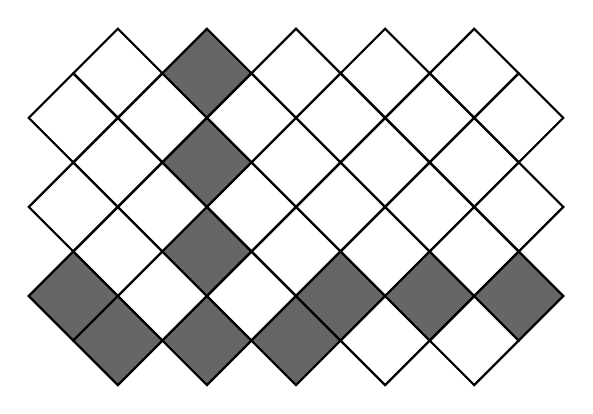
\begin{tikzpicture}[rotate=-45, scale=0.8]
        % row 1
        \cellb{2}{0}{3}{1}
        \cellb{3}{0}{4}{1}
        % row 2
        \cellw{1}{1}{2}{2}
        \cellw{2}{1}{3}{2}
        \cellw{3}{1}{4}{2}
        \cellb{4}{1}{5}{2}
        % row 3
        \cellw{0}{2}{1}{3}
        \cellw{1}{2}{2}{3}
        \cellw{2}{2}{3}{3}
        \cellb{3}{2}{4}{3}
        \cellw{4}{2}{5}{3}
        \cellb{5}{2}{6}{3}
        % row 4
        \cellw{0}{3}{1}{4}
        \cellw{1}{3}{2}{4}
        \cellb{2}{3}{3}{4}
        \cellw{3}{3}{4}{4}
        \cellw{4}{3}{5}{4}
        \cellb{5}{3}{6}{4}
        \cellw{6}{3}{7}{4}
        % row 5
        \cellb{1}{4}{2}{5}
        \cellw{2}{4}{3}{5}
        \cellw{3}{4}{4}{5}
        \cellw{4}{4}{5}{5}
        \cellw{5}{4}{6}{5}
        \cellb{6}{4}{7}{5}
        \cellw{7}{4}{8}{5}
        % row 6
        \cellw{2}{5}{3}{6}
        \cellw{3}{5}{4}{6}
        \cellw{4}{5}{5}{6}
        \cellw{5}{5}{6}{6}
        \cellw{6}{5}{7}{6}
        \cellb{7}{5}{8}{6}
        % row 7
        \cellw{3}{6}{4}{7}
        \cellw{4}{6}{5}{7}
        \cellw{5}{6}{6}{7}
        \cellw{6}{6}{7}{7}
        % row 8
        \cellw{4}{7}{5}{8}
        \cellw{5}{7}{6}{8}
    \end{tikzpicture}
\end{center}


This class has the following generating function.
$$C_3(x,y)=\frac{xy}{(1-x)^2(1-y)^2}+\frac{x^4 y^2}{(1-x)^3(1-y)}+\frac{x^2y^4}{(1-x)(1-y)^3}.$$
$$C_3(x,y)=\frac{xy}{(1-x)^2(1-y)^2}+\frac{x^4 y^2}{(1-x)^3(1-y)}+\frac{x^2y^4}{(1-x)(1-y)^3} - \frac{xy}{(1-x)^2} - \frac{xy}{(1-y)^2} + xy.$$

Note that we must add additional corrective terms the generating function of $c$, namely
$$C(x,y)=(C_0+C_1+C_2+C_3)(x,y) -\frac{x^2 y}{(1-x)^4} -\frac{x y^2}{(1-y)^4} + \frac{x^2+y}{1-x} + \frac{x+y^2}{1-y}-xy.$$

All polyforms not counted by $cc$ or $c$ are counted in $i$. $i$ can also be split into subclasses, namely $i_0,i_1,i_{1,1},r_1,i_2,i_3,i_4, i_5$, as well as the corrective term $r_3$ so that 
$$i(n,m)=(2i_{0}+4i_{1}+4i_{1,1}+r_1+2i_{2}+2i_{3}-r_3 + 4i_{4} + i_5)(n,m).$$

The subclass $i_0$ counts the number of polyforms of the following type
\begin{center}
    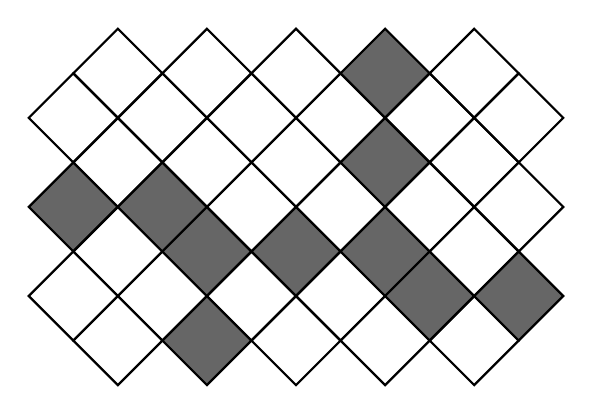
\begin{tikzpicture}[rotate=-45, scale=0.8]
        % row 1
        \cellw{2}{0}{3}{1}
        \cellw{3}{0}{4}{1}
        % row 2
        \cellb{1}{1}{2}{2}
        \cellw{2}{1}{3}{2}
        \cellw{3}{1}{4}{2}
        \cellb{4}{1}{5}{2}
        % row 3
        \cellw{0}{2}{1}{3}
        \cellw{1}{2}{2}{3}
        \cellb{2}{2}{3}{3}
        \cellb{3}{2}{4}{3}
        \cellw{4}{2}{5}{3}
        \cellw{5}{2}{6}{3}
        % row 4
        \cellw{0}{3}{1}{4}
        \cellw{1}{3}{2}{4}
        \cellw{2}{3}{3}{4}
        \cellw{3}{3}{4}{4}
        \cellb{4}{3}{5}{4}
        \cellw{5}{3}{6}{4}
        \cellw{6}{3}{7}{4}
        % row 5
        \cellw{1}{4}{2}{5}
        \cellw{2}{4}{3}{5}
        \cellw{3}{4}{4}{5}
        \cellw{4}{4}{5}{5}
        \cellb{5}{4}{6}{5}
        \cellb{6}{4}{7}{5}
        \cellw{7}{4}{8}{5}
        % row 6
        \cellw{2}{5}{3}{6}
        \cellw{3}{5}{4}{6}
        \cellb{4}{5}{5}{6}
        \cellw{5}{5}{6}{6}
        \cellw{6}{5}{7}{6}
        \cellb{7}{5}{8}{6}
        % row 7
        \cellb{3}{6}{4}{7}
        \cellw{4}{6}{5}{7}
        \cellw{5}{6}{6}{7}
        \cellw{6}{6}{7}{7}
        % row 8
        \cellw{4}{7}{5}{8}
        \cellw{5}{7}{6}{8}
    \end{tikzpicture}
\end{center}

\begin{equation*}
    i_0(n,m)= 2(n-1)(m-1) + \sum_{i=0}^{n-2}\sum_{j=0}^{m-2} (i+j)
\end{equation*}

\begin{equation*}
    I_0(x,y) = \sum_{n,m \geq 0}i_0(n,m)x^n y^m = \frac{2 x^2 y^2}{(1-x)^2 (1-y)^2} + \frac{x^3 y^2}{(1-x)^3(1-y)^2} + \frac{x^2 y^3}{(1-x)^2 (1-y)^3}
\end{equation*}

The subclass $i_1$ counts the number of polyforms of the following type

\begin{center}
    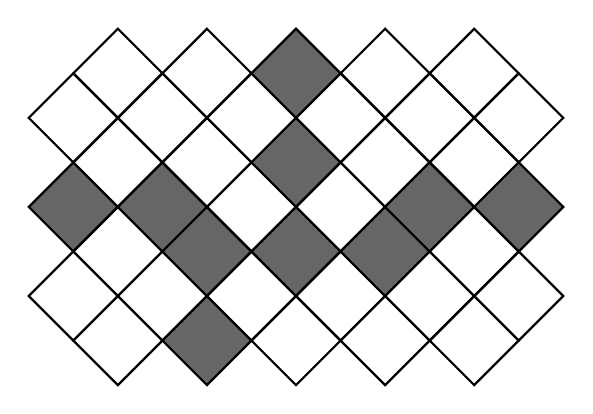
\begin{tikzpicture}[rotate=-45, scale=0.8]
        % row 1
        \cellw{2}{0}{3}{1}
        \cellw{3}{0}{4}{1}
        % row 2
        \cellb{1}{1}{2}{2}
        \cellw{2}{1}{3}{2}
        \cellw{3}{1}{4}{2}
        \cellb{4}{1}{5}{2}
        % row 3
        \cellw{0}{2}{1}{3}
        \cellw{1}{2}{2}{3}
        \cellb{2}{2}{3}{3}
        \cellb{3}{2}{4}{3}
        \cellw{4}{2}{5}{3}
        \cellw{5}{2}{6}{3}
        % row 4
        \cellw{0}{3}{1}{4}
        \cellw{1}{3}{2}{4}
        \cellw{2}{3}{3}{4}
        \cellw{3}{3}{4}{4}
        \cellb{4}{3}{5}{4}
        \cellw{5}{3}{6}{4}
        \cellw{6}{3}{7}{4}
        % row 5
        \cellw{1}{4}{2}{5}
        \cellw{2}{4}{3}{5}
        \cellb{3}{4}{4}{5}
        \cellw{4}{4}{5}{5}
        \cellb{5}{4}{6}{5}
        \cellw{6}{4}{7}{5}
        \cellw{7}{4}{8}{5}
        % row 6
        \cellb{2}{5}{3}{6}
        \cellw{3}{5}{4}{6}
        \cellw{4}{5}{5}{6}
        \cellb{5}{5}{6}{6}
        \cellw{6}{5}{7}{6}
        \cellw{7}{5}{8}{6}
        % row 7
        \cellw{3}{6}{4}{7}
        \cellw{4}{6}{5}{7}
        \cellw{5}{6}{6}{7}
        \cellb{6}{6}{7}{7}
        % row 8
        \cellw{4}{7}{5}{8}
        \cellw{5}{7}{6}{8}
    \end{tikzpicture}
\end{center}

\begin{equation*}
    I_1(x,y) = \sum_{n,m \geq 0} i_1(n,m)x^n y^m = C_1(x,y)\left(\frac{1}{(1-x)(1-y)}-1\right)
\end{equation*}

The subclass $i_{1,1}$ counts the number of polyforms of the following type

\begin{center}
    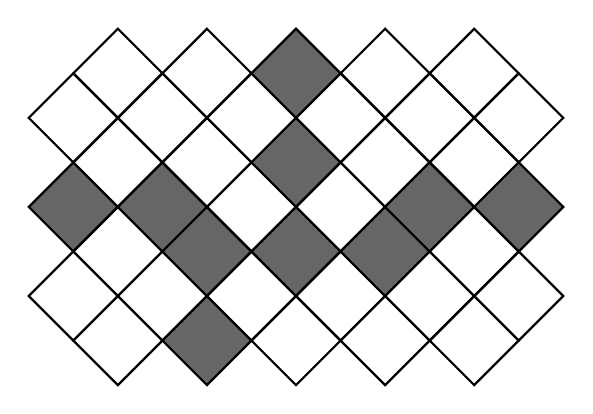
\begin{tikzpicture}[rotate=-45, scale=0.8]
        % row 1
        \cellw{2}{0}{3}{1}
        \cellw{3}{0}{4}{1}
        % row 2
        \cellb{1}{1}{2}{2}
        \cellw{2}{1}{3}{2}
        \cellw{3}{1}{4}{2}
        \cellb{4}{1}{5}{2}
        % row 3
        \cellw{0}{2}{1}{3}
        \cellw{1}{2}{2}{3}
        \cellb{2}{2}{3}{3}
        \cellb{3}{2}{4}{3}
        \cellw{4}{2}{5}{3}
        \cellw{5}{2}{6}{3}
        % row 4
        \cellw{0}{3}{1}{4}
        \cellw{1}{3}{2}{4}
        \cellw{2}{3}{3}{4}
        \cellw{3}{3}{4}{4}
        \cellb{4}{3}{5}{4}
        \cellw{5}{3}{6}{4}
        \cellw{6}{3}{7}{4}
        % row 5
        \cellw{1}{4}{2}{5}
        \cellw{2}{4}{3}{5}
        \cellb{3}{4}{4}{5}
        \cellw{4}{4}{5}{5}
        \cellb{5}{4}{6}{5}
        \cellw{6}{4}{7}{5}
        \cellw{7}{4}{8}{5}
        % row 6
        \cellb{2}{5}{3}{6}
        \cellw{3}{5}{4}{6}
        \cellw{4}{5}{5}{6}
        \cellb{5}{5}{6}{6}
        \cellw{6}{5}{7}{6}
        \cellw{7}{5}{8}{6}
        % row 7
        \cellw{3}{6}{4}{7}
        \cellw{4}{6}{5}{7}
        \cellw{5}{6}{6}{7}
        \cellb{6}{6}{7}{7}
        % row 8
        \cellw{4}{7}{5}{8}
        \cellw{5}{7}{6}{8}
    \end{tikzpicture}
\end{center}

\begin{equation*}
    I_{1,1}(x,y) = \sum_{n,m \geq 0} i_{1,1}(n,m)x^n y^m = \frac{2 x^2 y^3}{(1-x)^2 (1-y)^3} + \frac{2 x^3 y^2}{(1-x)^3 (1-y)^2 } + \frac{2x^2 y^4}{(1-x)^2 (1-y)^4} + \frac{2x^4 y^2}{(1-x)^4 (1-y)^2}
\end{equation*}

The corrective term $r_1$ counts all the polyforms in $i_1$ that are double counted when reflecting along both axes. An example polyform is below.

\begin{center}
    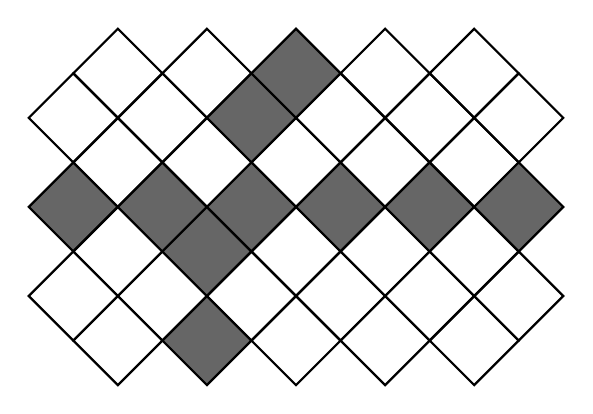
\begin{tikzpicture}[rotate=-45, scale=0.8]
        % row 1
        \cellw{2}{0}{3}{1}
        \cellw{3}{0}{4}{1}
        % row 2
        \cellb{1}{1}{2}{2}
        \cellw{2}{1}{3}{2}
        \cellw{3}{1}{4}{2}
        \cellb{4}{1}{5}{2}
        % row 3
        \cellw{0}{2}{1}{3}
        \cellw{1}{2}{2}{3}
        \cellb{2}{2}{3}{3}
        \cellb{3}{2}{4}{3}
        \cellw{4}{2}{5}{3}
        \cellw{5}{2}{6}{3}
        % row 4
        \cellw{0}{3}{1}{4}
        \cellw{1}{3}{2}{4}
        \cellw{2}{3}{3}{4}
        \cellb{3}{3}{4}{4}
        \cellw{4}{3}{5}{4}
        \cellw{5}{3}{6}{4}
        \cellw{6}{3}{7}{4}
        % row 5
        \cellw{1}{4}{2}{5}
        \cellb{2}{4}{3}{5}
        \cellw{3}{4}{4}{5}
        \cellb{4}{4}{5}{5}
        \cellw{5}{4}{6}{5}
        \cellw{6}{4}{7}{5}
        \cellw{7}{4}{8}{5}
        % row 6
        \cellb{2}{5}{3}{6}
        \cellw{3}{5}{4}{6}
        \cellw{4}{5}{5}{6}
        \cellb{5}{5}{6}{6}
        \cellw{6}{5}{7}{6}
        \cellw{7}{5}{8}{6}
        % row 7
        \cellw{3}{6}{4}{7}
        \cellw{4}{6}{5}{7}
        \cellw{5}{6}{6}{7}
        \cellb{6}{6}{7}{7}
        % row 8
        \cellw{4}{7}{5}{8}
        \cellw{5}{7}{6}{8}
    \end{tikzpicture}
\end{center}

\begin{equation*}
    R_1(x,y) = \sum_{n,m \geq 0} r_1(n,m)x^n y^m = \frac{2x^2 y^4}{(1-x)^4 (1-y)} + \frac{2x^4 y^2}{(1-x) (1-y)^4}
\end{equation*}

The subclass $i_2$ counts the number of polyforms of the following type

\begin{center}
    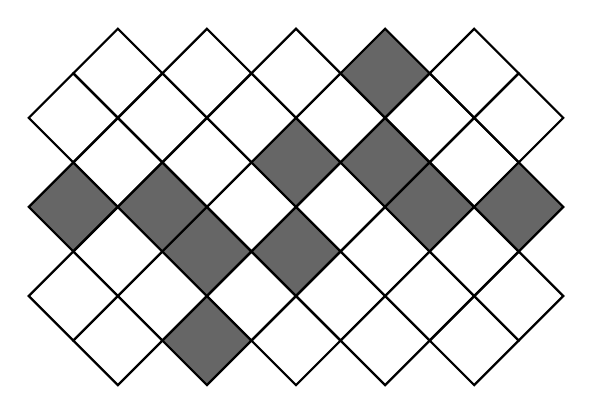
\begin{tikzpicture}[rotate=-45, scale=0.8]
        % row 1
        \cellw{2}{0}{3}{1}
        \cellw{3}{0}{4}{1}
        % row 2
        \cellb{1}{1}{2}{2}
        \cellw{2}{1}{3}{2}
        \cellw{3}{1}{4}{2}
        \cellb{4}{1}{5}{2}
        % row 3
        \cellw{0}{2}{1}{3}
        \cellw{1}{2}{2}{3}
        \cellb{2}{2}{3}{3}
        \cellb{3}{2}{4}{3}
        \cellw{4}{2}{5}{3}
        \cellw{5}{2}{6}{3}
        % row 4
        \cellw{0}{3}{1}{4}
        \cellw{1}{3}{2}{4}
        \cellw{2}{3}{3}{4}
        \cellw{3}{3}{4}{4}
        \cellb{4}{3}{5}{4}
        \cellw{5}{3}{6}{4}
        \cellw{6}{3}{7}{4}
        % row 5
        \cellw{1}{4}{2}{5}
        \cellw{2}{4}{3}{5}
        \cellb{3}{4}{4}{5}
        \cellw{4}{4}{5}{5}
        \cellw{5}{4}{6}{5}
        \cellw{6}{4}{7}{5}
        \cellw{7}{4}{8}{5}
        % row 6
        \cellw{2}{5}{3}{6}
        \cellw{3}{5}{4}{6}
        \cellb{4}{5}{5}{6}
        \cellb{5}{5}{6}{6}
        \cellw{6}{5}{7}{6}
        \cellw{7}{5}{8}{6}
        % row 7
        \cellb{3}{6}{4}{7}
        \cellw{4}{6}{5}{7}
        \cellw{5}{6}{6}{7}
        \cellb{6}{6}{7}{7}
        % row 8
        \cellw{4}{7}{5}{8}
        \cellw{5}{7}{6}{8}
    \end{tikzpicture}
\end{center}

\begin{eqnarray*}
    I_2(x,y) = \sum_{n,m\geq 0}i_2(n,m)x^n y^m & = & C_2(x,y)\left(\frac{1}{(1-x)(1-y)} -1\right) -\frac{x^3 y}{(1-x)^5} + \frac{x^2 y}{(1-x)^2} -\frac{x^2 y}{(1-x)} \\
    & - & \frac{x y^3}{(1-y)^5} + \frac{x y^2}{(1-y)^2} -\frac{x y^2}{(1-y)} - \frac{2x^2 y^2}{(1-x)^2 (1-y)^2} + \frac{2}{(1-x)(1-y)} \\
    & - & \frac{2xy+2}{1-x} - \frac{2xy + 2}{1-y} + 2xy + 2\\
\end{eqnarray*}


The subclass $i_3$ counts the number of polyforms of the following type

\begin{center}
    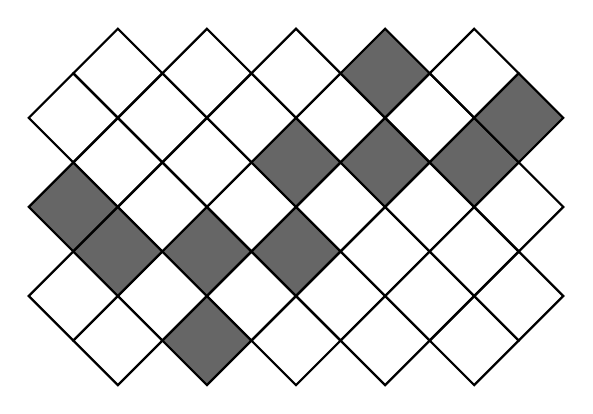
\begin{tikzpicture}[rotate=-45, scale=0.8]
        % row 1
        \cellw{2}{0}{3}{1}
        \cellw{3}{0}{4}{1}
        % row 2
        \cellb{1}{1}{2}{2}
        \cellb{2}{1}{3}{2}
        \cellw{3}{1}{4}{2}
        \cellb{4}{1}{5}{2}
        % row 3
        \cellw{0}{2}{1}{3}
        \cellw{1}{2}{2}{3}
        \cellw{2}{2}{3}{3}
        \cellb{3}{2}{4}{3}
        \cellw{4}{2}{5}{3}
        \cellw{5}{2}{6}{3}
        % row 4
        \cellw{0}{3}{1}{4}
        \cellw{1}{3}{2}{4}
        \cellw{2}{3}{3}{4}
        \cellw{3}{3}{4}{4}
        \cellb{4}{3}{5}{4}
        \cellw{5}{3}{6}{4}
        \cellw{6}{3}{7}{4}
        % row 5
        \cellw{1}{4}{2}{5}
        \cellw{2}{4}{3}{5}
        \cellb{3}{4}{4}{5}
        \cellw{4}{4}{5}{5}
        \cellw{5}{4}{6}{5}
        \cellw{6}{4}{7}{5}
        \cellw{7}{4}{8}{5}
        % row 6
        \cellw{2}{5}{3}{6}
        \cellw{3}{5}{4}{6}
        \cellb{4}{5}{5}{6}
        \cellw{5}{5}{6}{6}
        \cellw{6}{5}{7}{6}
        \cellw{7}{5}{8}{6}
        % row 7
        \cellb{3}{6}{4}{7}
        \cellw{4}{6}{5}{7}
        \cellb{5}{6}{6}{7}
        \cellw{6}{6}{7}{7}
        % row 8
        \cellw{4}{7}{5}{8}
        \cellb{5}{7}{6}{8}
    \end{tikzpicture}
\end{center}

\begin{eqnarray*}
    I_3(x,y) = \sum_{n,m \geq 0}i_3(n,m)x^n y^m & = & F(x,y)\left(\frac{4x^2 y^3}{(1-x)^2 (1-y)^4} + \frac{4x^3 y^2}{(1-x)^4 (1-y)^2}\right) \\
\end{eqnarray*}


The corrective term $r_3$ counts the number of polyforms in $i_3$ that are double-counted when reflecting along bothe axes. An example polyform is below.

\begin{center}
    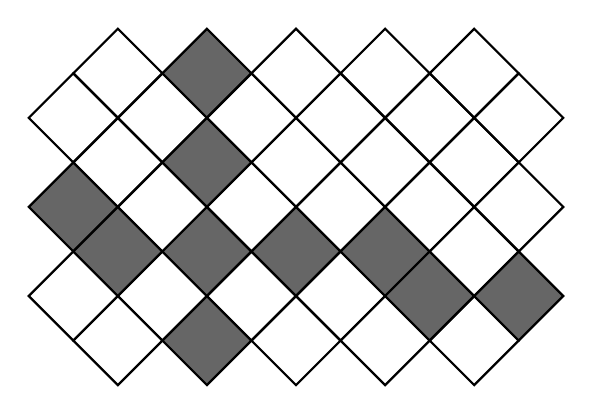
\begin{tikzpicture}[rotate=-45, scale=0.8]
        % row 1
        \cellw{2}{0}{3}{1}
        \cellw{3}{0}{4}{1}
        % row 2
        \cellb{1}{1}{2}{2}
        \cellb{2}{1}{3}{2}
        \cellw{3}{1}{4}{2}
        \cellb{4}{1}{5}{2}
        % row 3
        \cellw{0}{2}{1}{3}
        \cellw{1}{2}{2}{3}
        \cellw{2}{2}{3}{3}
        \cellb{3}{2}{4}{3}
        \cellw{4}{2}{5}{3}
        \cellw{5}{2}{6}{3}
        % row 4
        \cellw{0}{3}{1}{4}
        \cellw{1}{3}{2}{4}
        \cellb{2}{3}{3}{4}
        \cellw{3}{3}{4}{4}
        \cellb{4}{3}{5}{4}
        \cellw{5}{3}{6}{4}
        \cellw{6}{3}{7}{4}
        % row 5
        \cellb{1}{4}{2}{5}
        \cellw{2}{4}{3}{5}
        \cellw{3}{4}{4}{5}
        \cellw{4}{4}{5}{5}
        \cellb{5}{4}{6}{5}
        \cellb{6}{4}{7}{5}
        \cellw{7}{4}{8}{5}
        % row 6
        \cellw{2}{5}{3}{6}
        \cellw{3}{5}{4}{6}
        \cellw{4}{5}{5}{6}
        \cellw{5}{5}{6}{6}
        \cellw{6}{5}{7}{6}
        \cellb{7}{5}{8}{6}
        % row 7
        \cellw{3}{6}{4}{7}
        \cellw{4}{6}{5}{7}
        \cellw{5}{6}{6}{7}
        \cellw{6}{6}{7}{7}
        % row 8
        \cellw{4}{7}{5}{8}
        \cellw{5}{7}{6}{8}
    \end{tikzpicture}
\end{center}

\begin{equation*}
    R_3(x,y) = \sum_{n,m \geq 0} r_3(n,m) x^n y^m = \left(\frac{4x^2 y^3}{(1-x)^2 (1-y)^4} + \frac{4x^3 y^2}{(1-x)^4 (1-y)^2}\right)
\end{equation*}

The subclass $i_4$ counts the number of polyforms of the following type

\begin{center}
    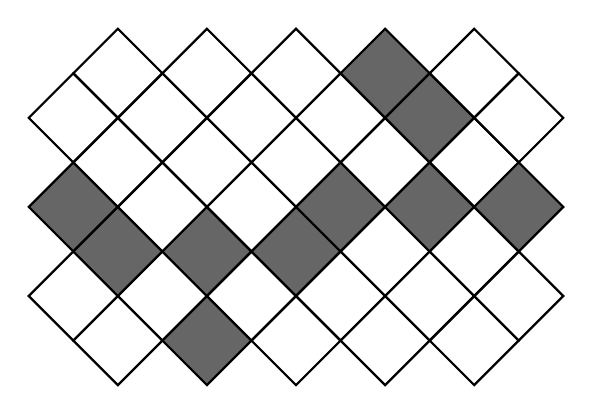
\begin{tikzpicture}[rotate=-45, scale=0.8]
        % row 1
        \cellw{2}{0}{3}{1}
        \cellw{3}{0}{4}{1}
        % row 2
        \cellb{1}{1}{2}{2}
        \cellb{2}{1}{3}{2}
        \cellw{3}{1}{4}{2}
        \cellb{4}{1}{5}{2}
        % row 3
        \cellw{0}{2}{1}{3}
        \cellw{1}{2}{2}{3}
        \cellw{2}{2}{3}{3}
        \cellb{3}{2}{4}{3}
        \cellw{4}{2}{5}{3}
        \cellw{5}{2}{6}{3}
        % row 4
        \cellw{0}{3}{1}{4}
        \cellw{1}{3}{2}{4}
        \cellw{2}{3}{3}{4}
        \cellw{3}{3}{4}{4}
        \cellb{4}{3}{5}{4}
        \cellw{5}{3}{6}{4}
        \cellw{6}{3}{7}{4}
        % row 5
        \cellw{1}{4}{2}{5}
        \cellw{2}{4}{3}{5}
        \cellw{3}{4}{4}{5}
        \cellb{4}{4}{5}{5}
        \cellw{5}{4}{6}{5}
        \cellw{6}{4}{7}{5}
        \cellw{7}{4}{8}{5}
        % row 6
        \cellw{2}{5}{3}{6}
        \cellw{3}{5}{4}{6}
        \cellw{4}{5}{5}{6}
        \cellb{5}{5}{6}{6}
        \cellw{6}{5}{7}{6}
        \cellw{7}{5}{8}{6}
        % row 7
        \cellb{3}{6}{4}{7}
        \cellb{4}{6}{5}{7}
        \cellw{5}{6}{6}{7}
        \cellb{6}{6}{7}{7}
        % row 8
        \cellw{4}{7}{5}{8}
        \cellw{5}{7}{6}{8}
    \end{tikzpicture}
\end{center}

\begin{eqnarray*}
    I_4(x,y) = \sum_{n,m \geq 0}i_4(n,m)x^n y^m & = & G(x,y)\left(\frac{4x^3 y^3}{(1-x)^3 (1-y)^3}\right) \\ 
\end{eqnarray*}

The subclass $i_5$ counts the number of polyforms of the following type

\begin{center}
    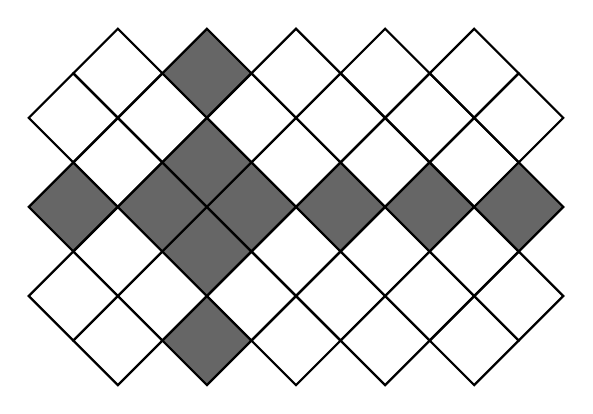
\begin{tikzpicture}[rotate=-45, scale=0.8]
        % row 1
        \cellw{2}{0}{3}{1}
        \cellw{3}{0}{4}{1}
        % row 2
        \cellb{1}{1}{2}{2}
        \cellw{2}{1}{3}{2}
        \cellw{3}{1}{4}{2}
        \cellb{4}{1}{5}{2}
        % row 3
        \cellw{0}{2}{1}{3}
        \cellw{1}{2}{2}{3}
        \cellb{2}{2}{3}{3}
        \cellb{3}{2}{4}{3}
        \cellw{4}{2}{5}{3}
        \cellw{5}{2}{6}{3}
        % row 4
        \cellw{0}{3}{1}{4}
        \cellw{1}{3}{2}{4}
        \cellb{2}{3}{3}{4}
        \cellb{3}{3}{4}{4}
        \cellw{4}{3}{5}{4}
        \cellw{5}{3}{6}{4}
        \cellw{6}{3}{7}{4}
        % row 5
        \cellb{1}{4}{2}{5}
        \cellw{2}{4}{3}{5}
        \cellw{3}{4}{4}{5}
        \cellb{4}{4}{5}{5}
        \cellw{5}{4}{6}{5}
        \cellw{6}{4}{7}{5}
        \cellw{7}{4}{8}{5}
        % row 6
        \cellw{2}{5}{3}{6}
        \cellw{3}{5}{4}{6}
        \cellw{4}{5}{5}{6}
        \cellb{5}{5}{6}{6}
        \cellw{6}{5}{7}{6}
        \cellw{7}{5}{8}{6}
        % row 7
        \cellw{3}{6}{4}{7}
        \cellw{4}{6}{5}{7}
        \cellw{5}{6}{6}{7}
        \cellb{6}{6}{7}{7}
        % row 8
        \cellw{4}{7}{5}{8}
        \cellw{5}{7}{6}{8}
    \end{tikzpicture}
\end{center}

\begin{equation*}
    I_5(x,y) = \sum_{n,m \geq 0} i_5(n,m) x^n y^m = \frac{xy}{(1-x)^2 (1-y)^2} - \frac{4x^2 y^2}{(1-x) (1-y)} - \frac{xy}{(1-x)^2} - \frac{xy}{(1-y)^2} + xy
\end{equation*}

which gives 

\begin{equation*}
    I(x,y) = (2I_0 + 4I_1 + 4I_{1,1} + R_1 + 2I_2 + 2I_3 - R_3 + 4I_4 + I_5)(x,y).
\end{equation*}

Introducing the following corrective term

\begin{equation*}
    T_r(x,y) = \frac{6x^2 y^2}{(1-x)^2 (1-y)} + \frac{6x^2 y^2}{(1-x) (1-y)^2}
\end{equation*}

allows us to write a full expression for the generating function, namely 

\begin{eqnarray*}
    \sum_{n,m \geq 0}\rho(A^{S^*}_{n,m})x^n y^m & = & (2CC + 4C + I - T_r)(x,y) + 2 +xy - \frac{4x}{(1-x)}- \frac{4y}{(1-y)} - \frac{2xy}{(1-x)^3} - \frac{2xy}{(1-y)^3} \\
    & + & \frac{(x+3x^2 -x^3 -x^4)y}{(1-x)^5} + \frac{(y+3y^2 -y^3 -y^4)x}{(1-y)^5}.\\
\end{eqnarray*}

This gives the result. 

\end{proof}


\end{document}
